\section{The X--\texorpdfstring{$\theta$}{theta} Mathematical Framework (Central Formalism)}\label{sec:framework}

I collect the full formalism here; later sections specialize to experiments and cosmology. To match prior drafts that used $F_{ab}$, I write the field strength on $Q$ as $G_{ab}\equiv\partial_aA_b-\partial_bA_a$ (synonymous with $F_{ab}$ earlier).

\paragraph{Units and conventions.} Unless stated otherwise, I use SI units in this section and keep $\hbar$ explicit in quantum contexts. In the relativistic Stueckelberg completion (\cref{sec:unified-force}) I adopt natural units with $\hbar=c=1$; when needed, $\hbar$ and $c$ can be restored by dimensional analysis.

\subsection{Configuration space, connection, and curvature}\label{sec:config-connection-curvature}
\begin{align}
Q&=\mathbb{R}^{3,1}\times S^1, & q^a&=(X^\mu,\theta), & a&\in\{0,1,2,3,\theta\},\\
A&=A_a\,dq^a= A_\mu\,dX^\mu + A_\theta\,d\theta, & G&=dA, & G_{ab}&=\partial_aA_b-\partial_bA_a.
\end{align}
Key mixed component: $G_{\mu\theta}=\partial_\mu A_\theta-\partial_\theta A_\mu$.

\begin{idea}
Think of ordinary space as a city map, and add a tiny circular \emph{dial} $\theta$ at every point. Turning the dial moves you along the fiber circle without moving on the map. The connection $A$ tells you how “phase” changes as you move—on the map and around the dial. The curvature $G=dA$ measures how those changes \emph{fail to cancel} around a loop (that failure is the holonomy). A picture of this "map\,$\times$\,dial" view is shown in Fig.~\ref{fig:map-dial}.
\end{idea}

\begin{figure}[h]
  \centering
  \includegraphics[width=\linewidth]{UG_S2_config_space_with_theta.png}
  \caption{Configuration space as “map $\times$ dial”: every base point carries a circular fiber $\theta$. Mixed curvature $G_{\mu\theta}$ links base motion to the fiber dial.}
  \label{fig:map-dial}
\end{figure}

\paragraph{Intuition and analogies.}
\begin{itemize}
  \item \textbf{Compact dimension ($S^1$).} $Q=\mathbb R^{3,1}\times S^1$ means I add one extra circular coordinate $\theta$ (angle, period $2\pi$) to ordinary space--time. Analogy: a garden hose looks 1D from afar but has a circular cross-section up close.
  \item \textbf{Gauge connection ($A$).} A geometric bookkeeping tool for how phases change when you move: a 1-form $A=A_a dq^a=A_\mu dX^\mu + A_\theta d\theta$. Analogy: a boat's navigation aid compensating for currents so transport is consistent.
  \item \textbf{Curvature ($G=dA$) and holonomy.} Curvature measures the failure of phase changes to cancel on a loop; holonomy is the loop-induced phase. Analogy: hike a loop around a hill and your compass heading can twist.
  \item \textbf{Mixed curvature ($G_{\mu\theta}$).} Couples base motion and internal rotation; in the common gauge $\partial_\theta A_\mu=0$ this reduces to a spatial gradient $\partial_\mu A_\theta$ that produces the cross-Hall response. Analogy: meshed gears---motion in one drives the other.
\end{itemize}

\subsection{Non-relativistic Lagrangian, Hamiltonian, and currents}\label{sec:nr-lagrangian}
With Newtonian time $t$ and $\phi\equiv A_0$,
\begin{align}
L_{\mathrm{NR}}&=\frac{m}{2}\dot X^2+\frac{I}{2}\dot\theta^2+q_X A_i\dot X^i+q_\theta A_\theta\dot\theta - q_X\,\phi,\\
P_i&=m\dot X^i+q_X A_i,\quad p_\theta=I\dot\theta+q_\theta A_\theta.
\end{align}
Equations of motion:
\begin{align}
m\ddot X_i &= q_X\big(E_i + (\dot{\bm X}\times\bm B)_i\big) + q_\theta\,G_{i\theta}\,\dot\theta,\\
I\ddot\theta &= q_\theta\,G_{\theta 0}+ q_\theta\,G_{\theta i}\,\dot X^i,
\end{align}
with $E_i=-\partial_tA_i-\partial_i\phi$ and $\bm B=\nabla\times\bm A$. Quantum dynamics on $Q$:
\begin{equation}
 i\hbar\,\partial_t\psi = \left[\frac{1}{2m}(-i\hbar\nabla_X-q_X\bm A)^2 + \frac{1}{2I}(-i\hbar\partial_\theta-q_\theta A_\theta)^2 + q_X\,\phi\right]\psi.
\end{equation}
Continuity on $Q$:
\begin{align}
 \partial_t\rho + \nabla_X\!\cdot\bm J_X + \partial_\theta J_\theta&=0,\\
 \bm J_X&=\frac{1}{m}\,\mathrm{Re}[\psi^\dagger(-i\hbar\nabla_X-q_X\bm A)\psi],\quad J_\theta=\frac{1}{I}\,\mathrm{Re}[\psi^\dagger(-i\hbar\partial_\theta-q_\theta A_\theta)\psi].
\end{align}

\begin{idea}
A Lagrangian is a \emph{trip budget}: kinetic terms are fuel costs (base and $\theta$ motion), potentials are hills, and the gauge potentials $(A_i,A_\theta)$ act like tolls that depend on where and how you move. The Hamiltonian is the accountant: it doesn’t let energy vanish, it just allows it to move between base motion, fiber motion, and interactions. A single units reminder keeps this honest: $[A_\theta]=\hbar/q_\theta$, so $q_\theta A_\theta$ carries momentum units along~$\theta$.
\end{idea}

\paragraph{Units sanity (quick check).}
\begin{itemize}
  \item $[A_\theta]=\hbar/q_\theta$ so that $q_\theta A_\theta$ carries momentum units along $\theta$; $[\partial_i A_\theta]= (\hbar/q_\theta)/\text{length}$.
  \item The Lagrangian piece $q_\theta A_\theta\,\dot\theta$ has energy units; the cross-Hall force term $q_\theta (\partial_i A_\theta)\,\dot\theta$ has force units.
\end{itemize}

\paragraph{Reading the Hamiltonian (at a glance).}
\begin{itemize}
  \item Minimal coupling: $\bm p\to \bm p - q_X\bm A$ and $p_\theta\to p_\theta - q_\theta A_\theta$ incorporate forces via potentials.
  \item Two kinetic energies describe base and fiber motion: $\tfrac{1}{2m}(\cdots)^2$ and $\tfrac{1}{2I}(\cdots)^2$. The parameter $I$ is an internal moment of inertia.
  \item Continuity on $Q$ is just probability conservation on the enlarged space.
\end{itemize}

\paragraph{EP hygiene (assumption).} To avoid composition-dependent violations of the equivalence principle at leading order, I take the $\theta$-charge to be composition-independent (e.g., $Q_\theta=\beta m$ or $\propto B\! -\!L$). This makes the new force universal at first approximation and is consistent with E\"otv\"os-type constraints; any residual composition dependence then only arises via the tiny portal mixings in \cref{sec:unified-force}.

Rotor spectrum and holonomy shift:
\begin{equation}
 E_\ell=\frac{\hbar^2}{2I}\Big(\ell-\frac{\phi_\theta}{2\pi}\Big)^2,\qquad \phi_\theta\equiv\frac{q_\theta}{\hbar}\oint A_\theta\,d\theta,\qquad \ell\in\mathbb Z.
\end{equation}

\subsection{Relativistic worldline, massless limit, and covariant wave equation}\label{sec:relativistic-worldline}
Worldline action with einbein $e(\tau)$ and metric $G^{(\mathrm{geom})}_{ab}dq^adq^b=\eta_{\mu\nu}dX^\mu dX^\nu+\kappa^2 d\theta^2$:
\begin{equation}
 S_{\mathrm{rel}}=\int d\tau\Big[\frac{1}{2e}\,G^{(\mathrm{geom})}_{ab}\,\dot q^a\dot q^b - \frac{e}{2}\,m^2 + q_X A_\mu\dot X^\mu + q_\theta A_\theta\dot\theta\Big].
\end{equation}
Mass-shell constraint $G^{ab}_{\mathrm{(geom)}}(P_a-q_aA_a)(P_b-q_bA_b)+m^2=0$. In the NR limit $I=m\kappa^2$.

\paragraph{Worldline and einbein (at a glance).}
\begin{itemize}
  \item The path is parametrized by $\tau$; the einbein $e(\tau)$ keeps the action reparametrization-invariant.
  \item Varying $e$ enforces the mass-shell condition that reduces to $E^2=\bm p^2+m^2$ when fields vanish.
  \item The added metric piece $\kappa^2 d\theta^2$ says motion in $\theta$ contributes to the worldline length; in the NR limit one finds $I=m\kappa^2$.
  \item Intuition: the einbein is like a choice of speedometer; it sets the clock along the path without changing the trip.
\end{itemize}

Covariant wave equation on $Q$ (scalar):
\begin{equation}
 \big[D_\mu D^\mu + \kappa^{-2} D_\theta^2 + m^2\big]\,\Psi(X,\theta)=0,\quad D_\mu=\partial_\mu+\tfrac{i}{\hbar}q_XA_\mu,\; D_\theta=\partial_\theta+\tfrac{i}{\hbar}q_\theta A_\theta.
\end{equation}

\paragraph{Massless limit (\texorpdfstring{$m\to 0$}{m->0}).} With finite $\kappa_0$,
\begin{equation}
 S_{m=0}=\int d\tau\Big[\frac{1}{2e}(\eta_{\mu\nu}\dot X^\mu\dot X^\nu+\kappa_0^2\dot\theta^2)+q_X A_\mu\dot X^\mu+q_\theta A_\theta\dot\theta\Big],\quad \eta_{\mu\nu}\dot X^\mu\dot X^\nu+\kappa_0^2\dot\theta^2=0.
\end{equation}

\paragraph{NR map.} Removing the rest-energy phase yields the Schr\"odinger equation in \cref{sec:nr-lagrangian} provided I identify $\boxed{\ I=m\kappa^2\ }$.

\begin{idea}
Two pictures: the \emph{rubber sheet} (curvature makes dimples that steer motion) and the \emph{ripple} (the covariant wave equation moves ripples consistently in any good coordinates). The fiber just adds one compact direction the ripple can wrap around; the NR limit packages it into the rotor inertia $I=m\kappa^2$.
\end{idea}

\paragraph{Parameter map.} The rotor inertia $I$ is a probe property tied to geometry via $I=m\kappa^2$, whereas the 4D vector mass $m_\theta=g_\theta f_\theta$ in the Stueckelberg completion is a mediator property controlling the shared Yukawa range $\lambda_\theta=1/m_\theta$ (\cref{sec:unified-force}).

\subsection{Gauge invariance on \texorpdfstring{$Q$}{Q} and large loops}\label{sec:gauge-invariance}
Gauge transformations: $A_\mu\to A_\mu+\partial_\mu\Lambda_X$, $A_\theta\to A_\theta+\partial_\theta\Lambda_\theta$, with $\psi\to \exp\!\left[-\tfrac{i}{\hbar}(q_X\Lambda_X+q_\theta\Lambda_\theta)\right]\psi$. Under a large gauge transformation around the circle, $\oint A_\theta d\theta \to \oint A_\theta d\theta + 2\pi\,\hbar/q_\theta$, so only $\phi_\theta$ modulo $2\pi$ is physical.

\begin{idea}
Changing gauge is like moving the zero mark on an altimeter: the mountain stays the same. Only \emph{closed loops} reveal structure. March once around the fiber circle and you collect a net phase $\phi_\theta=\tfrac{q_\theta}{\hbar}\oint A_\theta d\theta$, but physics cares only modulo $2\pi$ (large–gauge periodicity).
\end{idea}

\begin{figure}[h]
  \centering
  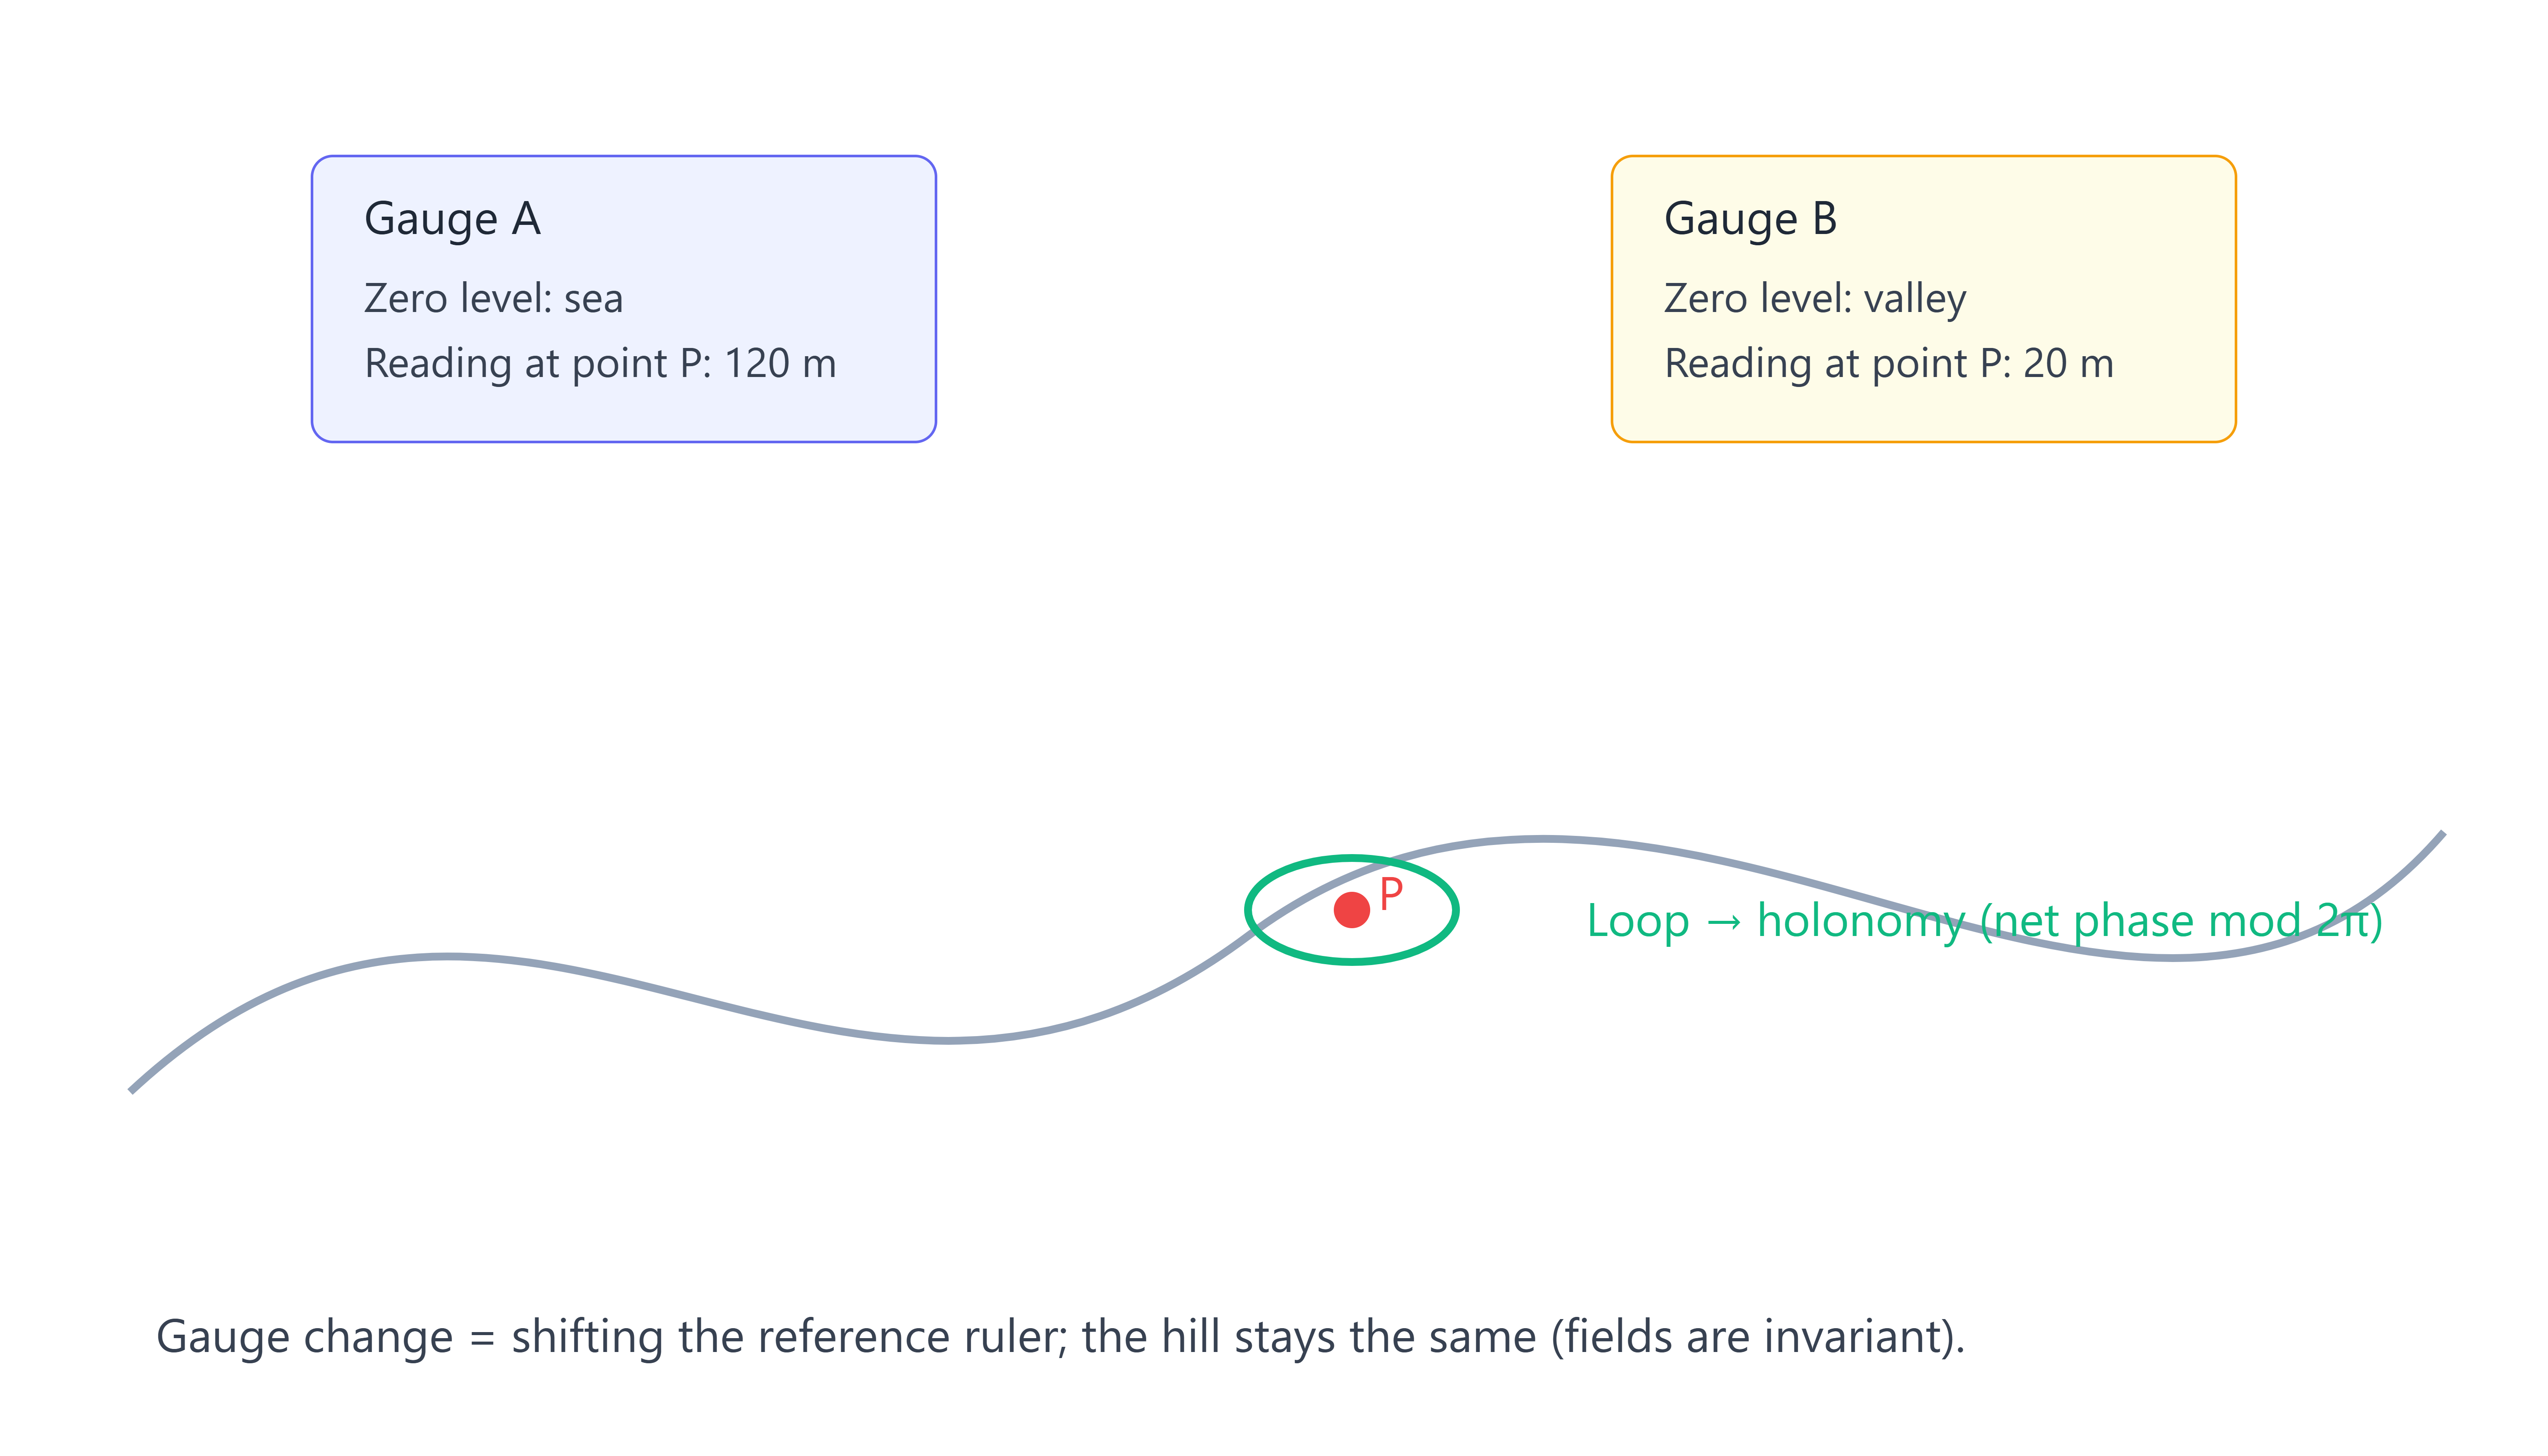
\includegraphics[width=\linewidth]{UG_S2_gauge_and_holonomy.png}
  \caption{Gauge change shifts the reference, not the hill. A closed loop probes holonomy; only $\phi_\theta\ (\bmod\ 2\pi)$ is observable.}
\end{figure}

The Bianchi identity $dG=0$ holds for $G=dA$ when one treats $(A_\mu, A_\theta)$ as components of a single connection; in many experiments I choose $\partial_\theta A_\mu=0$, leaving the measurable gradient $\partial_\mu A_\theta$.

\begin{figure}[h]
  \centering
  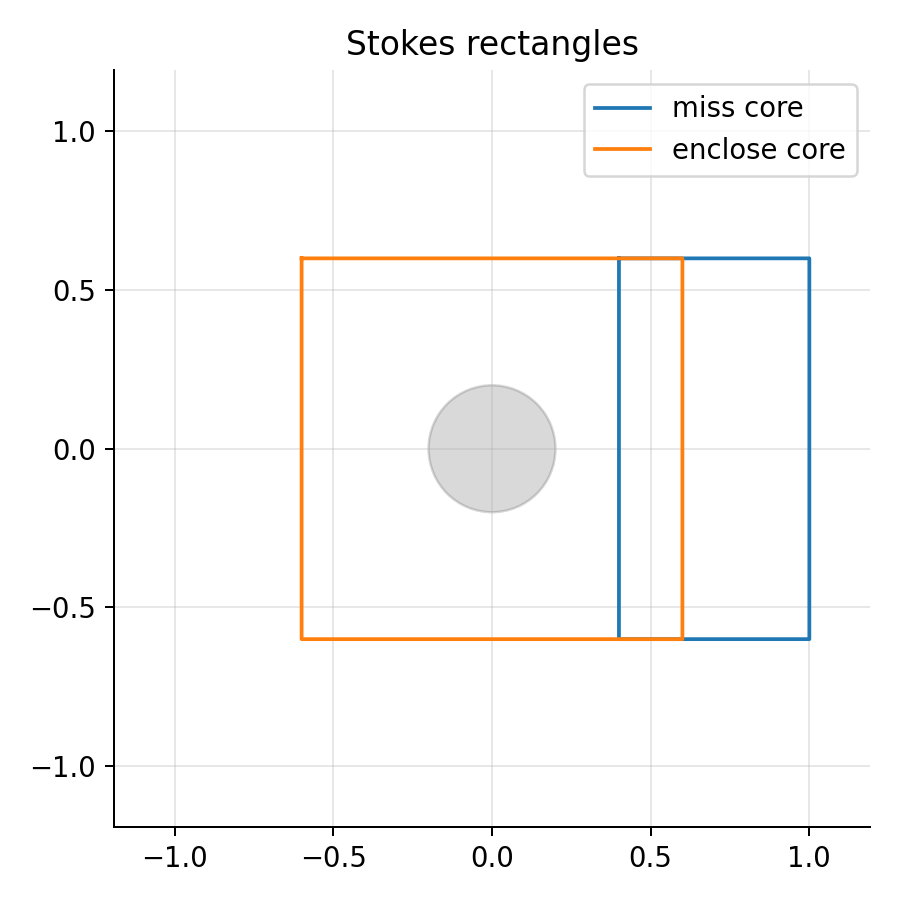
\includegraphics[width=0.6\linewidth]{stokes_rectangles.png}
  \caption{Holonomy schematic: Stokes rectangles visualize how loop integrals relate to enclosed curvature; only the loop integral modulo the large-gauge period is observable.}
  \label{fig:stokes}
\end{figure}

\subsection{Consistency checks \& known limits}\label{sec:consistency-checks}
\begin{itemize}
  \item \textbf{Turning off the fiber ($I\to\infty$, $q_\theta\to 0$).} Dynamics reduce to standard electrodynamics and quantum mechanics on $\mathbb R^{3,1}$: no $A_\theta$ phases and no rotor sidebands.
  \item \textbf{Turning off base electromagnetism ($q_X\to 0$).} The system is a free internal rotor that can still depend on $X$ through $A_\theta(X)$; sidebands with spacing $\Delta E\approx \hbar^2/(2I)$ and the $\theta$--AB phase $\Delta\phi_\theta=\tfrac{q_\theta}{\hbar}\oint A_\theta d\theta$ persist.
  \item \textbf{Relativistic $\to$ non-relativistic.} Identifying $I=m\kappa^2$ ensures the Schr\"odinger equation inherits the correct rotor term $\tfrac{1}{2I}(-i\hbar\partial_\theta-q_\theta A_\theta)^2$ after removing the rest-energy phase.
\end{itemize}

\subsection{Worked reductions (one screen)}\label{sec:worked-reductions}
I summarize the $I\to\infty$, $q_X\to 0$, and $I=m\kappa^2$ limits and their outcomes for observables (sidebands, holonomy) and consistency.
